\label{chapter:refactoring}
\chapter{Improving Software Metrics and Refactoring}
In Chapter \ref{chapter:problem-description}, the huge accumulated amount of technical debt in the system has been highlighted. A new robust and future-proof architecture has been proposed in Section \ref{chapter:architecture}. In this Chapter, the most important activities during the span of this thesis work will be presented. This includes a developer-friendly REST API and, a modern, simplistic and user-friendly grahical user interface, major important modifications to the available testing framework and refactoring of several components that can be found in Tribler. A summary of the refactoring efforts conducted is displayed in Table \ref{table:refactoring-summary}.\\\\

\begin{table}[h!]
	\centering
	\begin{tabular}{|l|l|}
		\hline
		\textbf{Lines modified} & 765 \\ \hline
		\textbf{Lines added} & 12.429 \\ \hline
		\textbf{Lines deleted (without GUI)} & 12.581 \\ \hline
		\textbf{Lines deleted (with GUI)} & 25.010 \\ \hline
	\end{tabular}
	\label{table:refactoring-summary}
	\caption{A summary of refactoring efforts as conducted during this thesis.}
\end{table}

\section{Improving tests and testability}
The most fundamental way to verify the correctness of software detect issues as soon as possible in the development cycles, is by having an exhaustive test suite. As described in Chapter \ref{chapter:problem-description}, the current test suite is plagued with unstable and non-functional tests. This section will discuss the performed work to strengthen and stabilize the test suite.

\subsection{Identifying Code Smells}
As described in the work of van Deursen et al\cite{van2001refactoring}, there is a difference between refactoring test code and production code in a sense that test code often has a characteristic set of code smells, originating from the way the tests are structured. Before we start to make major modifications to the test suite, we present a list of code smells identified in the test suite of Tribler. This list is visible in Table x.

\begin{table}
	\begin{tabularx}{\textwidth}{|X|X|X|}
		\hline
		\textbf{Code smell} & \textbf{Description} & \textbf{Solution}\\ \hline
		Dependency on external resources & Various tests are using external resources, leading to unpredictable and unstable tests. & Remove the dependency on the resource or make sure that the resource is locally available. \\ \hline
		State leak & The state of a previous executed test is leaking to the next test, mostly notable due to delayed calls left in the Twisted reactor. & Make sure that any delayed call in the reactor is removed when shutting down Tribler. \\ \hline
		Too much responsibility & Many tests have multiple responsibilities, testing both parts of the user interface and core components in Tribler. & Make sure that each test is only testing one unit in the system and design separate tests for the user interface.\\ \hline
		Slow tests & There are some slow tests (tests that are taking over 30 seconds to complete). This can be an indicator that the test is testing too much & Identify what is making the test slow and make the test as small as possible. \\ \hline
		Unclear assertions & Tests that have multiple assertions often do not annotate their assertion well with a clear and meaningful description & Add an explanation if an assertion fails.\\ \hline
		Dependency on a Tribler session & Some tests are starting a complete Tribler session while only a small subset of the system is tested & Use mocking techniques to inject a mocked session or refactor the component so no session is required. \\ \hline
		Resource writing to the source directory & Various tests are writing resources to the source code directory. They might accidentally end up in the VCS if developers are not cautious. & Temporary resources produced by tests should be written to a temporary directory that is correctly cleaned after test execution. \\ \hline
		Claiming the same local port & Some tests that are running in parallel are claiming the same local port, leading to test failures. & Reserve port ranges to individual parallel test runs. \\ \hline
		Timing issues & Various tests are checking a condition after a fixed interval. This interval is often based on intuition rather than empirical data. This is particularly dangerous when the test is dependent on external resources. & Refactor the test so the condition check is no longer necessary.\\ \hline
		No usage of comments & There are no comments, explaining what the the tests are testing and what the expected output is. & Comments should be added with a description of the test. \\ \hline
	\end{tabularx}
	\caption{Identified code smells in the test suite of Tribler as of November '15.}
	\label{table:tests-code-smells}
\end{table}

\subsection{Improving Code Coverage}
Code coverage is defined as the percentage of source code that is covered by at least one test in the test suite. Our continuous integration environment offers tools to track the code coverage over time. After each automated test suite execution a comprehensive report with detailed information about the code coverage is generated. The reported metrics by this report are not accurate enough since some third-party libraries are included in the coverage report, such as the VLC bindings and \emph{pymdht}, a library to fetch peers from the Distributed Hash Table (DHT). Also, the code coverage of Dispersy is included in these reports while we consider Dispersy as a separate engineering project.\\\\
The difference in code coverage during the span of this thesis can be found in Table \ref{table:code-coverage-table}. Branch coverage is a metric that specifies how well conditional statements are covered. This metric includes the fact that a conditional is either resolved to true or false, possibly influencing the program execution path. In the ideal scenario, we wish to have tests that cover all conditional statements in the case they resolve to \emph{true} and in the case they resolve to \emph{false} so we cover all possible execution paths in the program. This objective gets significantly harder to achieve when code with many nested conditional statements is written. The cyclomatic complexity as developed by McCabe in 1976\cite{mccabe1976complexity} is a quantitative measure of the number of linear independent paths through a program's source code. Any conditional written has a negative effect on the cyclomatic complexity.\\\\
While at first sight it may look like the code coverage has not increased significantly, we should emphasize that the complete architecture of the tests have been overhauled in parallel. Refactoring of the test suite had consequences on the code coverage in other locations in the code base. For instance, the smaller unit tests are not starting the old user interface, leading to a lower coverage in that module.\\\\
Improving the code coverage has been done by writing small unit tests where we are using mocked objects to have better control over the system we are testing. Using mocking in Tribler is a necessary since some components have many other dependencies that are hard to keep under control without using custom, controlled objects. Libtorrent is a good example of this. During this thesis, many unit tests have been written as can be seen in Figure x where the number of unit tests over time is presented. Writing tests makes a developer more aware of the written code and can be a good way to get familiar with an unknown system. Due to this, various bugs have been solved during the process of writing additional tests.

\begin{table}
	\begin{tabular}{ l | l | l | l | l | }
		\cline{2-5}
		& \multicolumn{2}{ | c | }{\textbf{November '15}} &
		\multicolumn{2}{ | c | }{\textbf{July '16} }\\
		\cline{2-5}
		& Lines coverage & Branch coverage & Lines coverage & Branch coverage\\ \hline
		\multicolumn{1}{|l|}{Core} & 71,2\% & 58,1\% & 81,2\% & 67,3\%\\ \hline
		\multicolumn{1}{|l|}{REST API} & - & - & 99,4\% & 92,7\%\\ \hline
		\multicolumn{1}{|l|}{wx GUI} & 65,8\% & 42,7\% & - & -\\ \hline
		\multicolumn{1}{|l|}{Qt GUI} & - & - & 70,0\% & x\\ \hline
	\end{tabular}
	\caption{The difference in code coverage between November '15 and July '16.}
	\label{table:code-coverage-table}
\end{table}

\begin{figure}[h!]
	\centering
	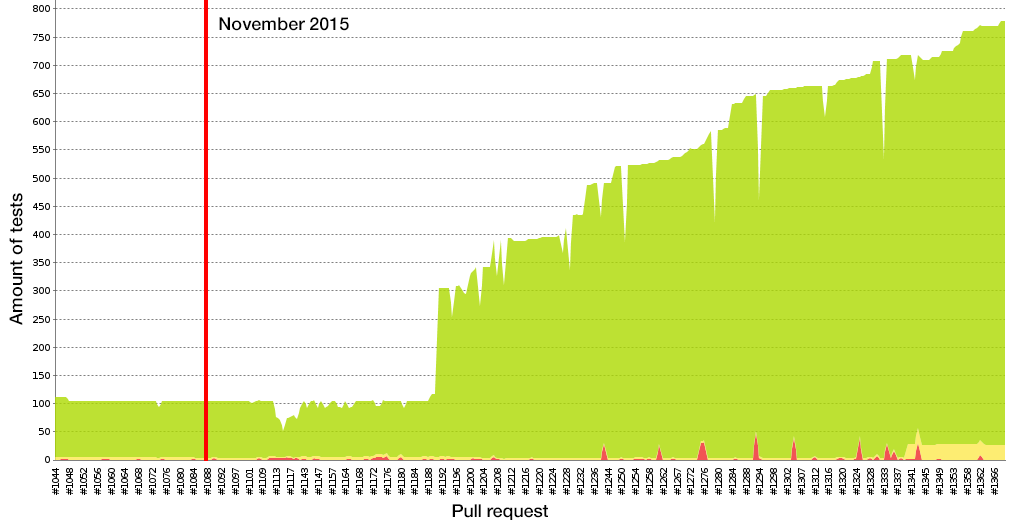
\includegraphics[width=0.8\columnwidth]{images/improving_qa/test_trend}
	\caption{The number of tests over time.}
	\label{fig:importgraph-qt-gui}
\end{figure}

In Chapter \ref{chapter:problem-description}, Figure \ref{fig:tests-ratio-tribler} we presented the ratio between the number of code lines in the tests package and the amount of other code lines over time. Together with the code coverage, this number can be a useful metric to developers. While one might argue that having a high code coverage in conjunction with a low TLC/PLC ratio is a desired result, it indicates that the tests are not granular enough and are actually doing many different operations. A low code coverage with a high TLC/PLC ratio indicates that there are some flaws in the tests, possibly that they are testing the wrong components of the system. When starting the thesis, Tribler has a low code coverage together with a low TLC/PLC ratio\todo{beter uitleggen}.\\\\
After writing additional unit tests, removal of the old user interface and addition of the new one, the new ratio is \emph{0.16} which means that there is roughly one line of test code for six lines of other source code in Tribler. Defining a good TLC/PLC ratio is dependent on the used programming language, development methodology and application structure. Discussion on the wiki of Ward Cunningham\cite{c2tlcratio} proposes an optional ratio of 1:1, however, several other ratios have been proposed on the same page such as 2:1 and 5:1. In the work described in \cite{van2001refactoring}, an ideal ratio of 1:1 is proposed. Overall, the trend seems to be that the amount of test line code is around the same or a bit higher than the lines of production code. An important question is whether this proposed ratio also holds for Tribler. Tribler differs from a commercial software engineering project in the sense that it is used for scientific research. When performing research, it is easy to ignore testing and focus on the results that are gathered by the system. The difficulty here is that Tribler is distributed and used by over a million of users, requiring at least some form of quality assurance. We think a better optional TLC/PLC ratio for the Tribler project might be 1:2.\\\\
To make sure that the responsibility of code coverage is not neglected in future work on Tribler, an addition check for each pull request has been added that verifies that the code contributed in the respective pull request is covered by tests. While not created by the author of this thesis, this check is an effective way to keep the code coverage metric under control.

\subsection{Testing the New User Interface}
One of the issues in the old testing framework, was that there is no clear separation between tests that are testing the user interface and tests that are testing core functionalities of Tribler. This is one of the reasons that have led to big, extensive tests in the old test suite. Since testing is an important aspect of this thesis work, writing proper tests for the user interface has been a prioritized task earlier in the development process of the new user interface.\\\\
GUI testing is an interesting area in the field of software engineering and is part of the application testing methodology. GUI testing can also be more involving than unit testing since a user interface might have many different operations\todo{afmaken, cites etc}.\\\\
Testing the new Qt user interface makes use of the \emph{QTest} framework. This framework provides various tools to perform non-blocking waits and to  simulate mouse clicks and keyboard actions. A sample of a test written with the \emph{QTest} framework is illustrated in Listing \ref{lst:qtest-sample}. After the interface is started, the test navigates to the home page, clicks on the \emph{channels} tab button and waits for items to be loaded. During the test execution, two screenshots are captured, one when we are loading items and another one when the requested items are loaded and displayed.\\\\
Primitives to capture screenshots during test execution has already been implemented and used in the old test suite, using the rendering engine of \emph{wxPython}. The \emph{Qt} frameworks offers similar tools. Captured screenshots are exported to \emph{jpg} files under a name specified by the developer. In the sample given in Listing \ref{lst:qtest-sample}, the exported screenshots are saved as \emph{screenshot\_home\_page\_channels\_loading.jpg} and \emph{screenshot\_home\_page\_channels.jpg} respectively. At the end of each test run, an image gallery is generated where the generated screenshots are archived and displayed in a grid. This allows developers to manually verify whether visual elements are correctly displayed. A part of the generated image gallery is displayed in Figure \ref{fig:jenkins-gallery}.

\begin{figure}[h!]
	\centering
	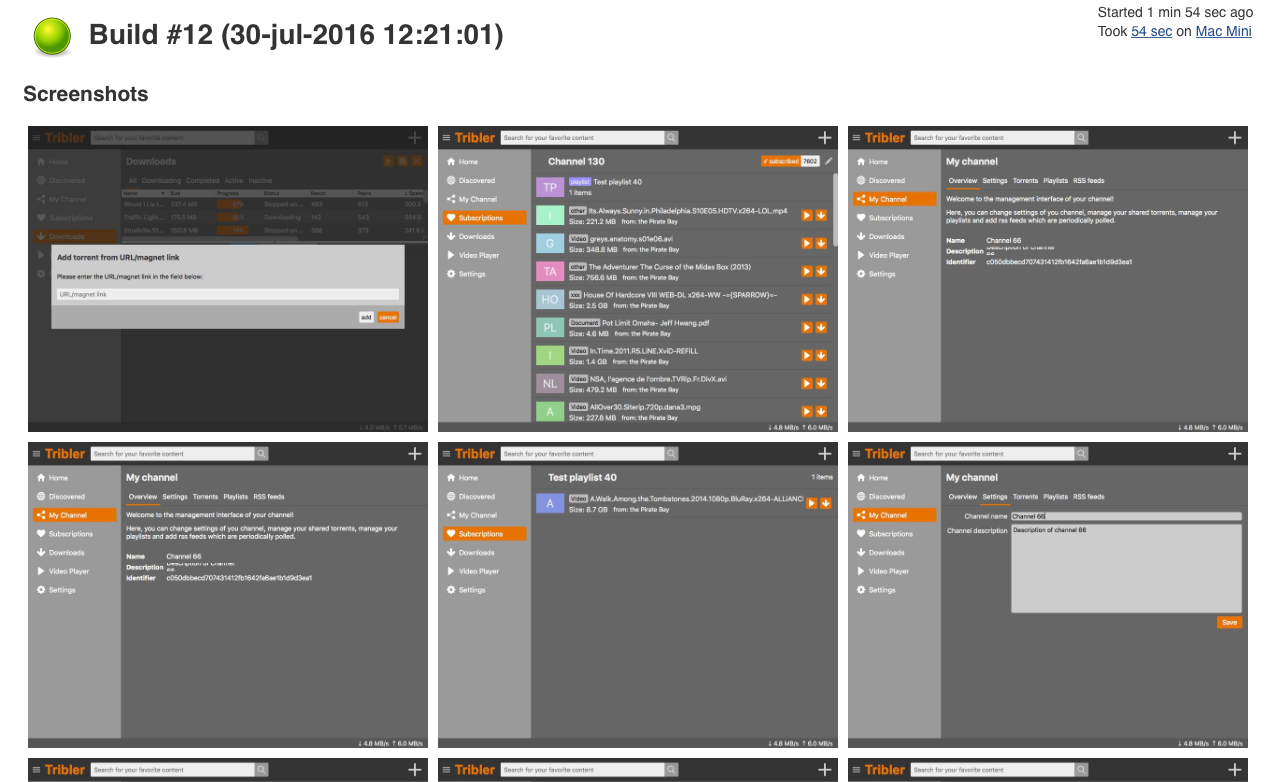
\includegraphics[width=1.0\columnwidth]{images/improving_qa/gallery_jenkins}
	\caption{The generated image gallery after executing of the user interface tests, generated by Jenkins.}
	\label{fig:jenkins-gallery}
\end{figure}

To avoid dependencies on Tribler itself and thus re-introducing the problem we are trying to solve, we created a small piece of software that provides the same interface as the REST API implemented. This 'fake' API is much simpler in nature and has a very simplistic in-memory data model. The downside of this approach is that new endpoints have to be written twice, once in Tribler and once in this fake API, providing that the new endpoint will covered by a user interface test.

\begin{lstlisting}[caption={A sample of a test that tests the new Qt Tribler GUI.},label={lst:qtest-sample}]
def test_home_page_channels(self):
	QTest.mouseClick(window.left_menu_button_home, Qt.LeftButton)
	QTest.mouseClick(window.home_tab_channels_button, Qt.LeftButton)
	self.screenshot(window, name="home_page_channels_loading")
	self.wait_for_home_page_table_populated()
	self.screenshot(window, name="home_page_channels")
\end{lstlisting}

\subsection{External Network Resources}
On of the problems with the test suite was that dependencies on external network resources should either be removed or one should verify that the resources are under the control of the developer and always available. The test suite contains various tests where external torrent files are fetched from the internet, in particular, from the Ubuntu repository. While this repository can guarantee high availability, any downtime in this external resource can lead to failing tests. The implemented solution for this design flaw is to start up a local HTTP server that serves the torrent file. While this approach requires more code to manage this local server, it completely removes the dependency on the Ubuntu repository.\\\\
The same solution has been applied to solve the dependency on external seeders. A small number of tests makes assumptions on the availability of torrent pieces of the network. This certainly makes tests fail if the executing machines has a bad or even no internet connection. The process of setting up a local seeder session is straightforward. Again, this approach requires code to properly start and shut down the seeder session. The implementation is reusable to an extend that developers of tests can reuse the implemented solutions with only a few lines of code.\\\\
Unfortunately, there are some external network dependencies left which are considered harder to refactor. A handful of tests are performing a remote keyword search, requiring various communities in Dispersy to be loaded. These tests are dependent on available peers in the respective community in order to make sure there are incoming search results. The proposed solution here is to start various dedicated Dispersy sessions on the local machine. Due to time constraints, the implementation of this solution is considered future work.

\subsection{Instability of Tests}
Well-designed tests should only fail if some new code is breaking existing functionality. If no changes are presents, the tests should always succeed. Reducing dependencies on external network is not sufficient to guarantee this in Tribler. The structural problem of the tests is that the system is infested with race conditions. Race conditions can be invisible since they often occur in a very specific runtime setting of the system, making the debugging process of these kind of errors frustrating.\\\\
During this thesis, many race conditions have been detected and solved. One interesting observation is that some issues only occurred on a specific platform. We believe can be explained by differences in the implementation of underlying threading model across operating systems. The most common cause of failing tests can be addressed to delayed calls in the Twisted reactor. During the test execution, Tribler is restarted many times. If a developer leaves by accident a delayed call behind when the shut down procedure has been completed, this delayed call might be executed in the wrong Tribler session, possibly leading to an inconsistent state of the system. Making sure the reactor is completely clean is not straightforward: if one is not aware of scheduled calls in the system, the mistake is easily made.\\\\
Writing stable tests also requires the test to be limited in what they do. Each test should only be focussed on the specific part of the system that has to be tested\todo{cite?}. While often unnecessary, a significant amount of the available tests are focused on starting a complete Tribler session, testing a small subset of the system, and shutting down Tribler again. While this approach is relatively easy to code, starting a fully-fledged session often leads to more instability and unexpected side-effects during test execution. Instead, only the classes to be tested should be instantiated and any dependencies this class have, should be mocked. Mocking ensures that developers have control over dependencies, allowing them to specify any expected return value. Moreover, the execution time of these small unit tests is significantly lower than the tests where a Tribler session is managed. The additional unit tests that have been written during this thesis, are following the described design.

\subsection{Continuous Integration Enhancements}
Tribler makes use of the popular continuous integration (CI) platform Jenkins. Jenkins allows developers to define jobs which can be executed manually or when pushing a commit on the code base. This continuous integration platform is responsible for running the tests, packaging Tribler and running research-oriented experiments.\\\\
When we focus on the execution of the tests, it is immediately noticed that they are only executed in a Linux environment. Beller et al\cite{beller2016oops} conducted research on CI adoption and usage and it turned out that for some languages, it might benefit to run tests in different environment. An addition argument for this is the usage of many platform-specific workarounds we are using in Tribler. To make sure that these statements are covered, we must run the tests in this environment. This will allow developers to detect defects on other platforms more earlier in the development process. By aggregating the generated coverage report on each platform, this multi-platform setup should benefit the code coverage.\\\\
The setup of the testing environments on Windows and OS X is straightforward. New slave nodes to specify the Windows and OS X test runners have been created. The tests on OS X are executed on a Mac Mini\todo{specs}. In order to run the tests on Windows, two virtual machines using Proxmox have been created, both 32-bit and 64-bit environments. In total, the tests are executed on four platforms now: Linux, Windows 32-bit, Windows 64-bit and OS X. So far, the OS X and Windows test executers have completed over 2.500 test runs. Each test runner generates a coverage reports and these reports are merged in the final analyse step in the build pipeline.\\\\
While this is certainly a step in the right direction, there are various additional steps in the execution plan that can be performed. In Figure \ref{fig:jenkins-pipeline}, the ideal test execution plan is displayed, together with the various stages in this pipeline. We start by executing the tests on multiple platforms where during these runs, the code coverage is being tracked. After this phase, the coverage reports are combined and the total difference with the upstream branch is determined. When the commit decreases the total code coverage, the job fails.\\\\
A static Pylint checker has been available to check for code style violations, however this only gave insight in the total amount of Pylint errors and did not stimulate to actually fix errors in the committed code. While not implemented by the author of this thesis, the Pylint checker has been extended to fail if new violations are introduced in the committed code. Additionally, a report is generated with an overview of the introduced violations. This helps developers to get more aware of the code style. This checker is ran in parallel with the tests to decrease the total time of the pipeline execution.\\\\
After the coverage phase has passed, jobs to package Tribler for distribution should be added. In parallel, the \emph{AllChannel} experiment can be executed. This experiment is executed on the DAS5 supercomputer and starts 1.000 Tribler clients that are synchronizing torrents and channels with each other. When the experiment is completed, several graphs are generated, providing developers insights in the consequences of their modified code when Tribler runs in a more comprehensive environment. For instance, the experiment can highlight issues in the message synchronization between peers in the network.\\\\
In parallel with the \emph{AllChannel} experiment, we can package Tribler for distribution to end-users. On Windows, an installer will be created that installs Tribler to the \emph{Program Files}. On OS X, we create a \emph{DMG} file that contains an app bundle. On Linux, the required files are bundled in a \emph{deb} archive. All these jobs can be executed in parallel. Finally, we should test whether the final distributions are working. This should be achieved by executing the final Tribler executable. A small test suite that makes use of the REST API can be created.

\begin{figure}[h!]
	\centering
	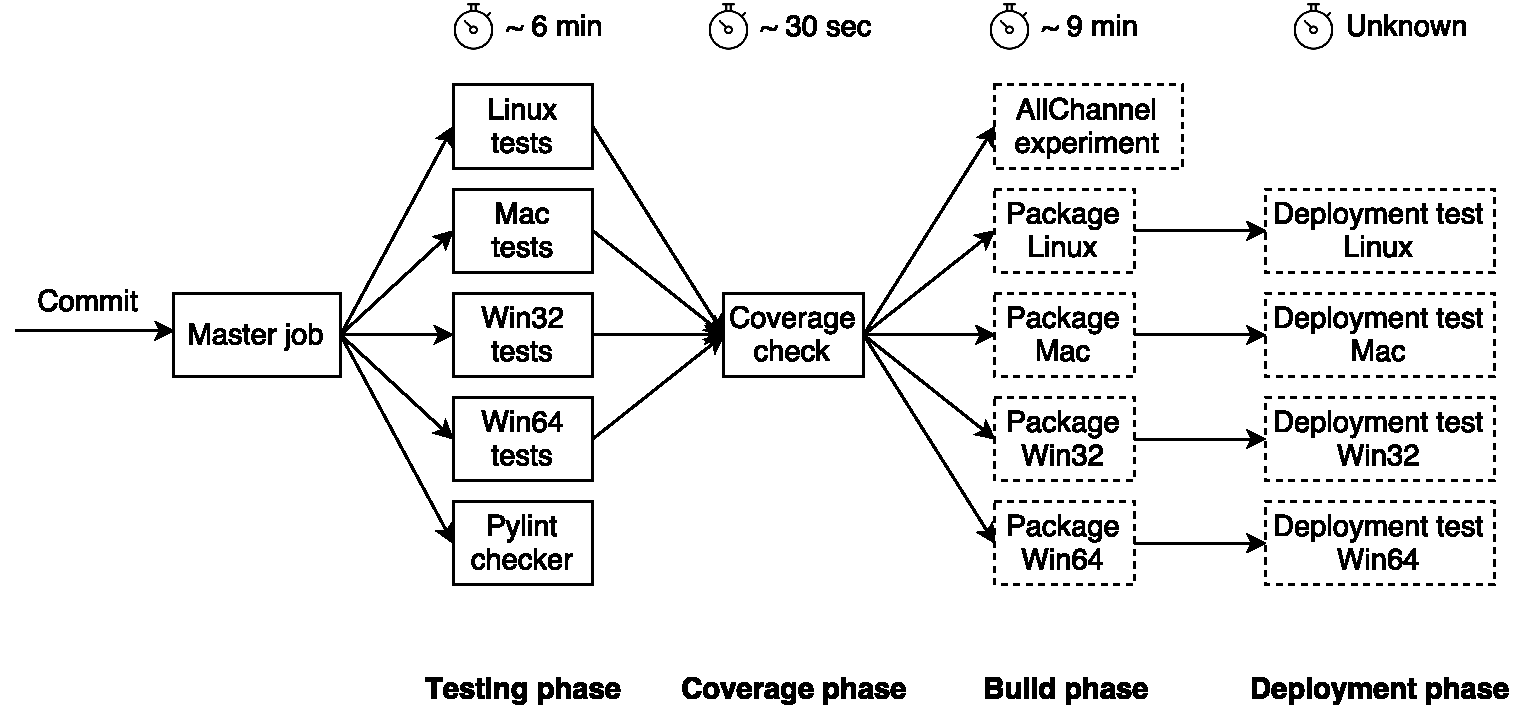
\includegraphics[width=0.9\columnwidth]{images/improving_qa/jenkins_pipeline}
	\caption{The desired test execution plan in our continuous integration environment. Dashed boxes are not implemented yet.}
	\label{fig:jenkins-pipeline}
\end{figure}

\section{REST API}
As described in Chapter \ref{chapter:architecture}, communication between the graphical user interface and the Tribler core is facilitated using a REST API. This Section explains the implementation of the API in more detail.\\\\
The REST API is written using Twisted. While there are plenty of Python libraries available that allow developers to facilitating a web server in their application, Twisted is used since it already represents a big part of the internal structure of Tribler. With the possibility to integrate the REST API into the main application flow, we avoid having to create special constructions to run the API for instance on a separate thread. API endpoints in Twisted are represented as a resource tree. This is in accordance with REST where the URL of the request can be treated like a path in the resource tree. This structure is also visible to some extent in the import graph of the API module as displayed in Figure \ref{fig:importgraph-api}. We will highlight and discuss some important files in the API module:
\begin{itemize}
	\item \emph{rest\_manager}: the \emph{rest\_manager} file contains the \emph{RESTManager} class which is responsible for starting and stopping the API. In addition, this file contains the \emph{RESTRequest} class which is a subclass of \emph{server.Request} (which in turn is instantiated by Twisted on an incoming request) and handles any exceptions that occurred during the serving of the HTTP request.
	\item \emph{root\_endpoint}: this file hosts the \emph{RootEndpoint} class which represents the root node of our resource tree. This class dispatches incoming requests to the right sub nodes in the tree.
	\item \emph{util}: the \emph{util} file contains various helper functions, such as conversion utilities to easily transform channel and torrent data from the database into JSON format that can be sent to the client that initiated a request.
\end{itemize}

\begin{figure}[h!]
	\centering
	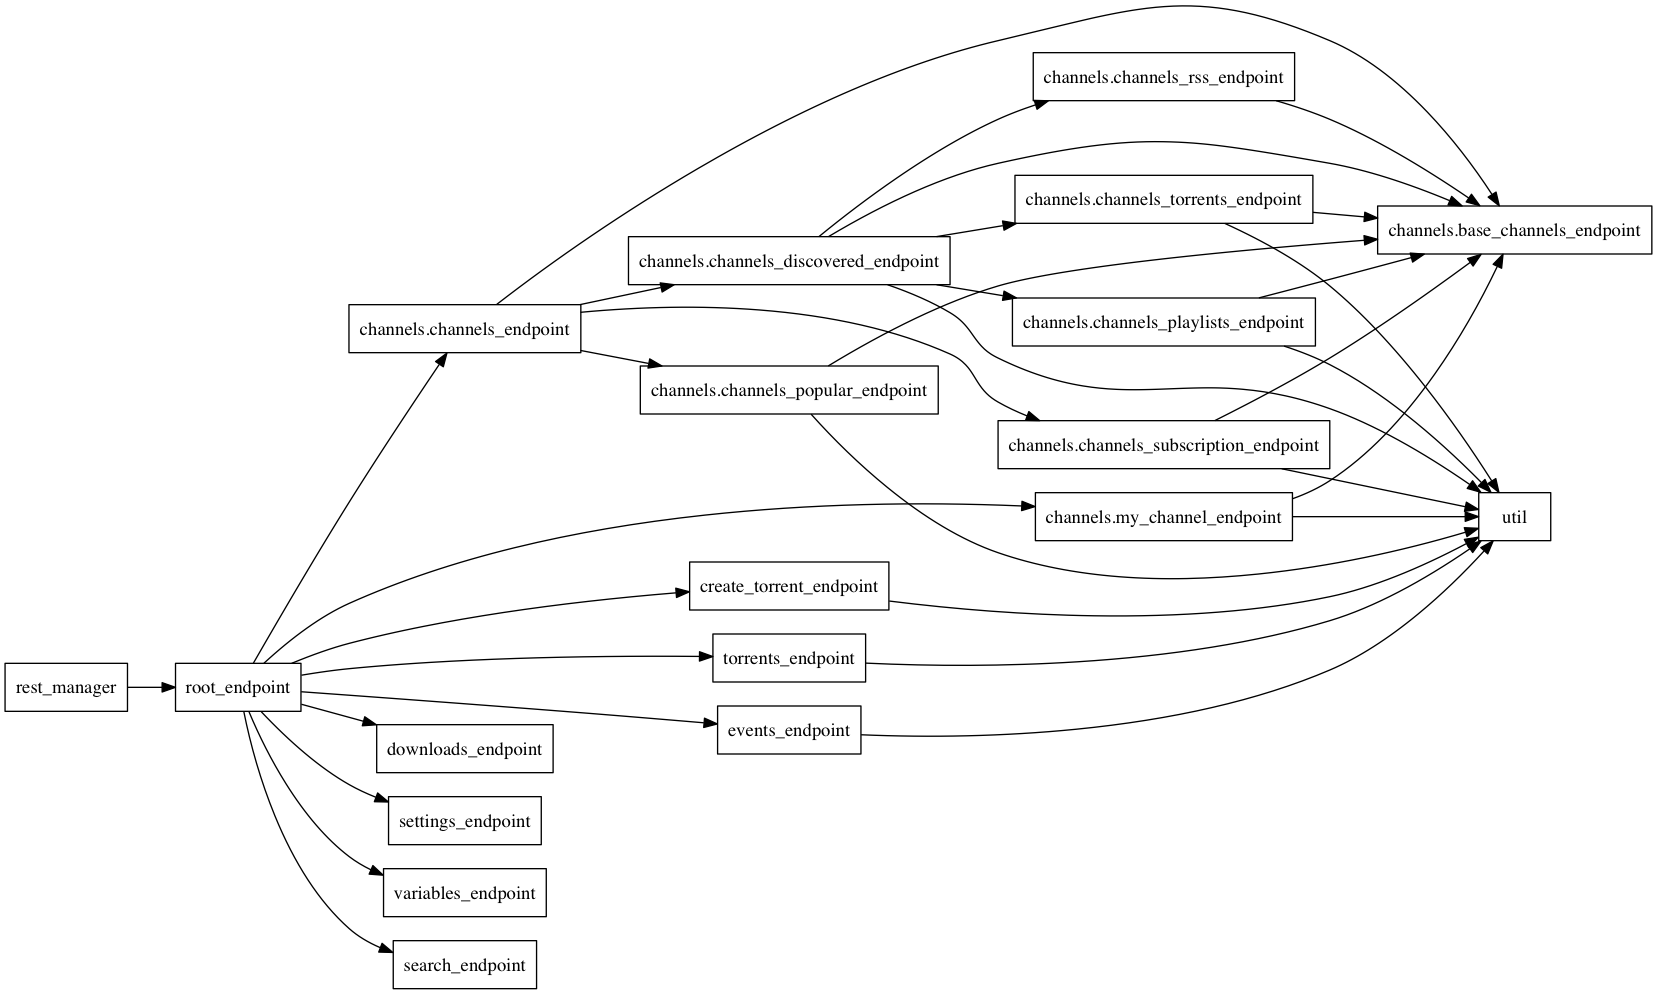
\includegraphics[width=1.0\columnwidth]{images/improving_qa/importgraph_api}
	\caption{The import graph of the REST API module.}
	\label{fig:importgraph-api}
\end{figure}

Except for some endpoints, all data returned by the API is structured in JSON format. The JSON format is well adopted in the field of web engineering and easy to parse. Most of the endpoints are straightforward implementations where the client performs a request and some data is returned. There are situations where the client does a request and a stream of data should be returned. For instance, this is the case when the user performs a search query. Sometimes, data should be returned to the client, even if the client did not ask for this data. When a crash in the Tribler core code occurred, the client should be notified of this crash and possibly warn the user that he or she should restart the application. For this purpose, an asynchronous events stream has been designed and created. Clients can open this event stream and interesting notifications are sent over this stream. All messages that are sent over the \emph{events} connection are shown in Table \ref{table:rest-api-events}.\\

\begin{table}
\begin{tabularx}{\textwidth}{|l|X|}
	\hline
	\textbf{Event name} & \textbf{Description} \\ \hline
	\emph{events\_start} & The events connection is opened and the server is ready to send events.  \\ \hline
	\emph{search\_result\_channel} & Tribler received a channel search result (either remote or locally). The event contains the channel result data. \\ \hline
	\emph{search\_result\_torrent} & Tribler received a torrent search result (either remote or locally). The event contains the torrent result data. \\ \hline
	\emph{upgrader\_started} & The Tribler upgrader started. \\ \hline
	\emph{upgrader\_tick} & The status of the Tribler upgrader changed. This event contains a human-readable string with the status update. \\ \hline
	\emph{upgrader\_finished} & The Tribler upgrader finished. \\ \hline
	\emph{watch\_folder\_corrupt\_torrent} & The watch folder module has encountered a corrupt .torrent file. The name of the file is part of this emitted event.\\ \hline
	\emph{new\_version\_available} & A new version of Tribler is available. The version number is contained in the event.\\ \hline
	\emph{tribler\_started} & Tribler has completed the startup procedure and is ready to serve HTTP requests on all endpoints.\\ \hline
	\emph{channel\_discovered} & A new channel has been discovered. The events contains the discovered channel data.\\ \hline
	\emph{torrent\_discovered} & A new torrent has been discovered. The events contains the discovered torrent data.\\ \hline
\end{tabularx}
\caption{An overview of all events that are passed over the asynchronous events connection, part of the REST API.}
\label{table:rest-api-events}
\end{table}

The API is started in two stages. Just before starting Tribler, the \emph{events} connection is activated. This connection is initialized earlier so we can send interesting updates of the upgrader to the client. When the upgrader is completed and Tribler has been started, the other endpoints are activated and the API is ready to be used.

\section{Graphical User Interface}
The amount of accumulated technical debt in the current graphical user interface of Tribler is devastating. After going through several development cycles where some impacting changes have been made, the code base of the user interface has reached the point where it is more beneficial to create a complete new user interface. This section will continue the discussion that has been initiated in Section \ref{chapter:problem-description}. First, the structure of the current user interface will be described. Next, the new interface, introduced in Chapter \ref{chapter:architecture} will be elaborated. Encountered design decisions and challenges are presented and discussed.

\subsection{The current user interface}
\todo{Better title} The current user interface is unintuitive and cluttered with widgets and many functionality that should be in the core module of Tribler, can be found at higher levels in the user interface code. There is actually no clear separation between the core and the user interface, making it hard for developers to develop and test new functionalities since they have to deal with a bigger code base. One of the goals of this thesis is to make this separation more explicit for developers so they do not have to touch interface-related code if they are not interested in that.\\\\
The code base of the user interface is full of undesired workarounds and code smells. There is no clear, documented structure to be identified throughout the code and there are several reasons for this issue. One of the underlying causes is the mindset of developers that the user interface code base is subordinate to the code related to the core functionalities of Tribler. While it is often true that minor defects in the user interface are less critical than errors in important core functionalities such as the download engine, developer should always strive to write maintainable code. The fact that the user interface has undergone dramatic changes throughout the 10 years of research is an additional reason that led to this unstructured code base. Making short-term decisions were clearly favoured over decisions that benefit the longer-term development process.\\\\
If we take a closer look at the structure of the user interface code base, several files with many class definitions can be found. In the \emph{widgets.py} file, we can identify 30 distinct widget definitions. The \emph{SearchGridManager} file acts like the glue between the Tribler core and the user interface. Most of the requests to the core are passing through method definitions inside this file.

\subsection{Building a new user interface}
Before starting to create a new user interface, we should first decide which graphical user interface library we would like to use. There are plenty of libraries that are suited for this job. Below, several of such libraries are summarized, together with a small description and some (dis)advantages.
\begin{itemize}
	\item \emph{wxPython}: this is the current user interface library we are using. \emph{wxPython} is built upon \emph{wxWidgets} and provides the Python bindings to this latter library. The library is cross-platform and we can continue to use \emph{wxPython}. We already have a large code base written in \emph{wxPython} so continued usage of this library could allow us to reuse several widgets. The main disadvantages of this library are the minor inconsistencies across different platforms and the lack of a visual designer, requiring us to specify the complete layout in Python code.
	\item \emph{Kivy}: the cross-platform library Kivy has been used by Tribler research, particularly in the past attempts to run Tribler on Android\cite{de2014android}\cite{sabee2014tribler}. The decision of using Kivy for the new user interface enables us to reuse the interface logic on Android. The layout of Kivy can either be created in \emph{.kv} files or specified in code which is based on the separation of concerns principle. While not as old as \emph{wxPython} or \emph{pyQt}, the library has gained significant attention and adoption in the Python community.
	\item \emph{TKinder}: the \emph{TKinder} library is a layer built upon the Tcl/Tk framework and is considered the de-facto graphical user interface library for Python. Like the other discussed frameworks, \emph{TKinder} does not provide a visual designer. The library is built-in in Python which means that no additional libraries have to be installed in order to start writing code. \emph{TKinder} however is considered more suitable for simple applications due to the simplistic nature of the library.
	\item \emph{PyQt}: \emph{PyQt} provides the Python bindings for the Qt framework and is widely used in open-source and commercial applications. With a first version released in 1995, the Qt framework has evolved into a mature state. The library is very well documentation and provides many different addons and plugins to support a wide range of applications. One of these plugins is a visual WYSIWYG designer where the layout of an interface can be specified in a drag-and-drop manner. This generates a \emph{xml} file which can be read and parsed by \emph{Qt}. Visual styles can be specified using the  \emph{Cascading Style Sheet} (CSS) language. The documentation of \emph{Qt} is very comprehensive, although the documentation regarding \emph{PyQt} is somewhat less maintained.
\end{itemize}
Since the graphical user interface will be an important aspect of Tribler, we wish to use a library that is future-proof, well-maintained and easy to use. We think that in the context of this thesis, choosing \emph{PyQt} is the best choice to build a new user interface. The fact that we can specify our layout using an editor is an enormous advantage since this will mean that we have less code to contribute. In addition, this allows other developers that are not familiar with the Tribler code base to contribute to the graphical user interface. The \emph{Qt} visual designer also offers tools for internationalization and translation of the interface in foreign languages. Tasks like these are perfect opportunities for contributions in an open source project and can potentially attract new developers. A screenshot of the used visualizer is visible in Figure x.\\\\
The result of the development of the new interface is displayed in Figure \ref{fig:new-gui-1}. The majority of the new user interface has been built using the visual designer. Some code has been written to handle requests to the Tribler core, display the right data in lists and to manage interface-related settings. Connections between widgets and Python code are made using the signal-slot mechanism in \emph{Qt}. This mechanism is used for communication between objects and is a central feature in the \emph{Qt} framework. Widgets in \emph{Qt} can have signals, events they want to possibly notify to other widgets. Some widgets have some built-in signals, i.e. a button emits a \emph{clicked} signal if the user clicks the button with the mouse. Other widgets or Python objects can subscribe to these signals. These signals and slots can either be specified using code or the visual designer, however, to keep the amount of Python code to be maintained to a minimum, we decided to specify our widgets connections in the visual designer as much as possible.\\

\begin{figure}[t]
	\centering
	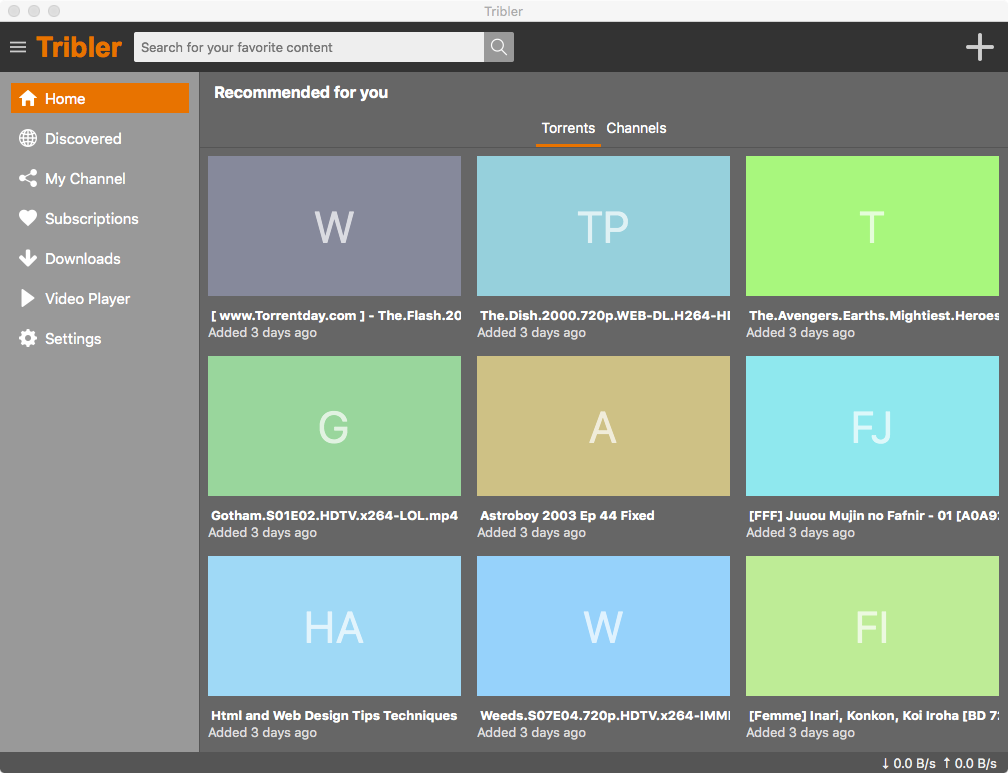
\includegraphics[width=0.8\columnwidth]{images/improving_qa/newgui1}
	\caption{The home page of the new user interface.}
	\label{fig:new-gui-1}
\end{figure}

During development of the user interface, some issues that required some careful analysis were encountered. The remained of the Section will describe these issues in more detail.

\begin{figure}[h!]
	\centering
	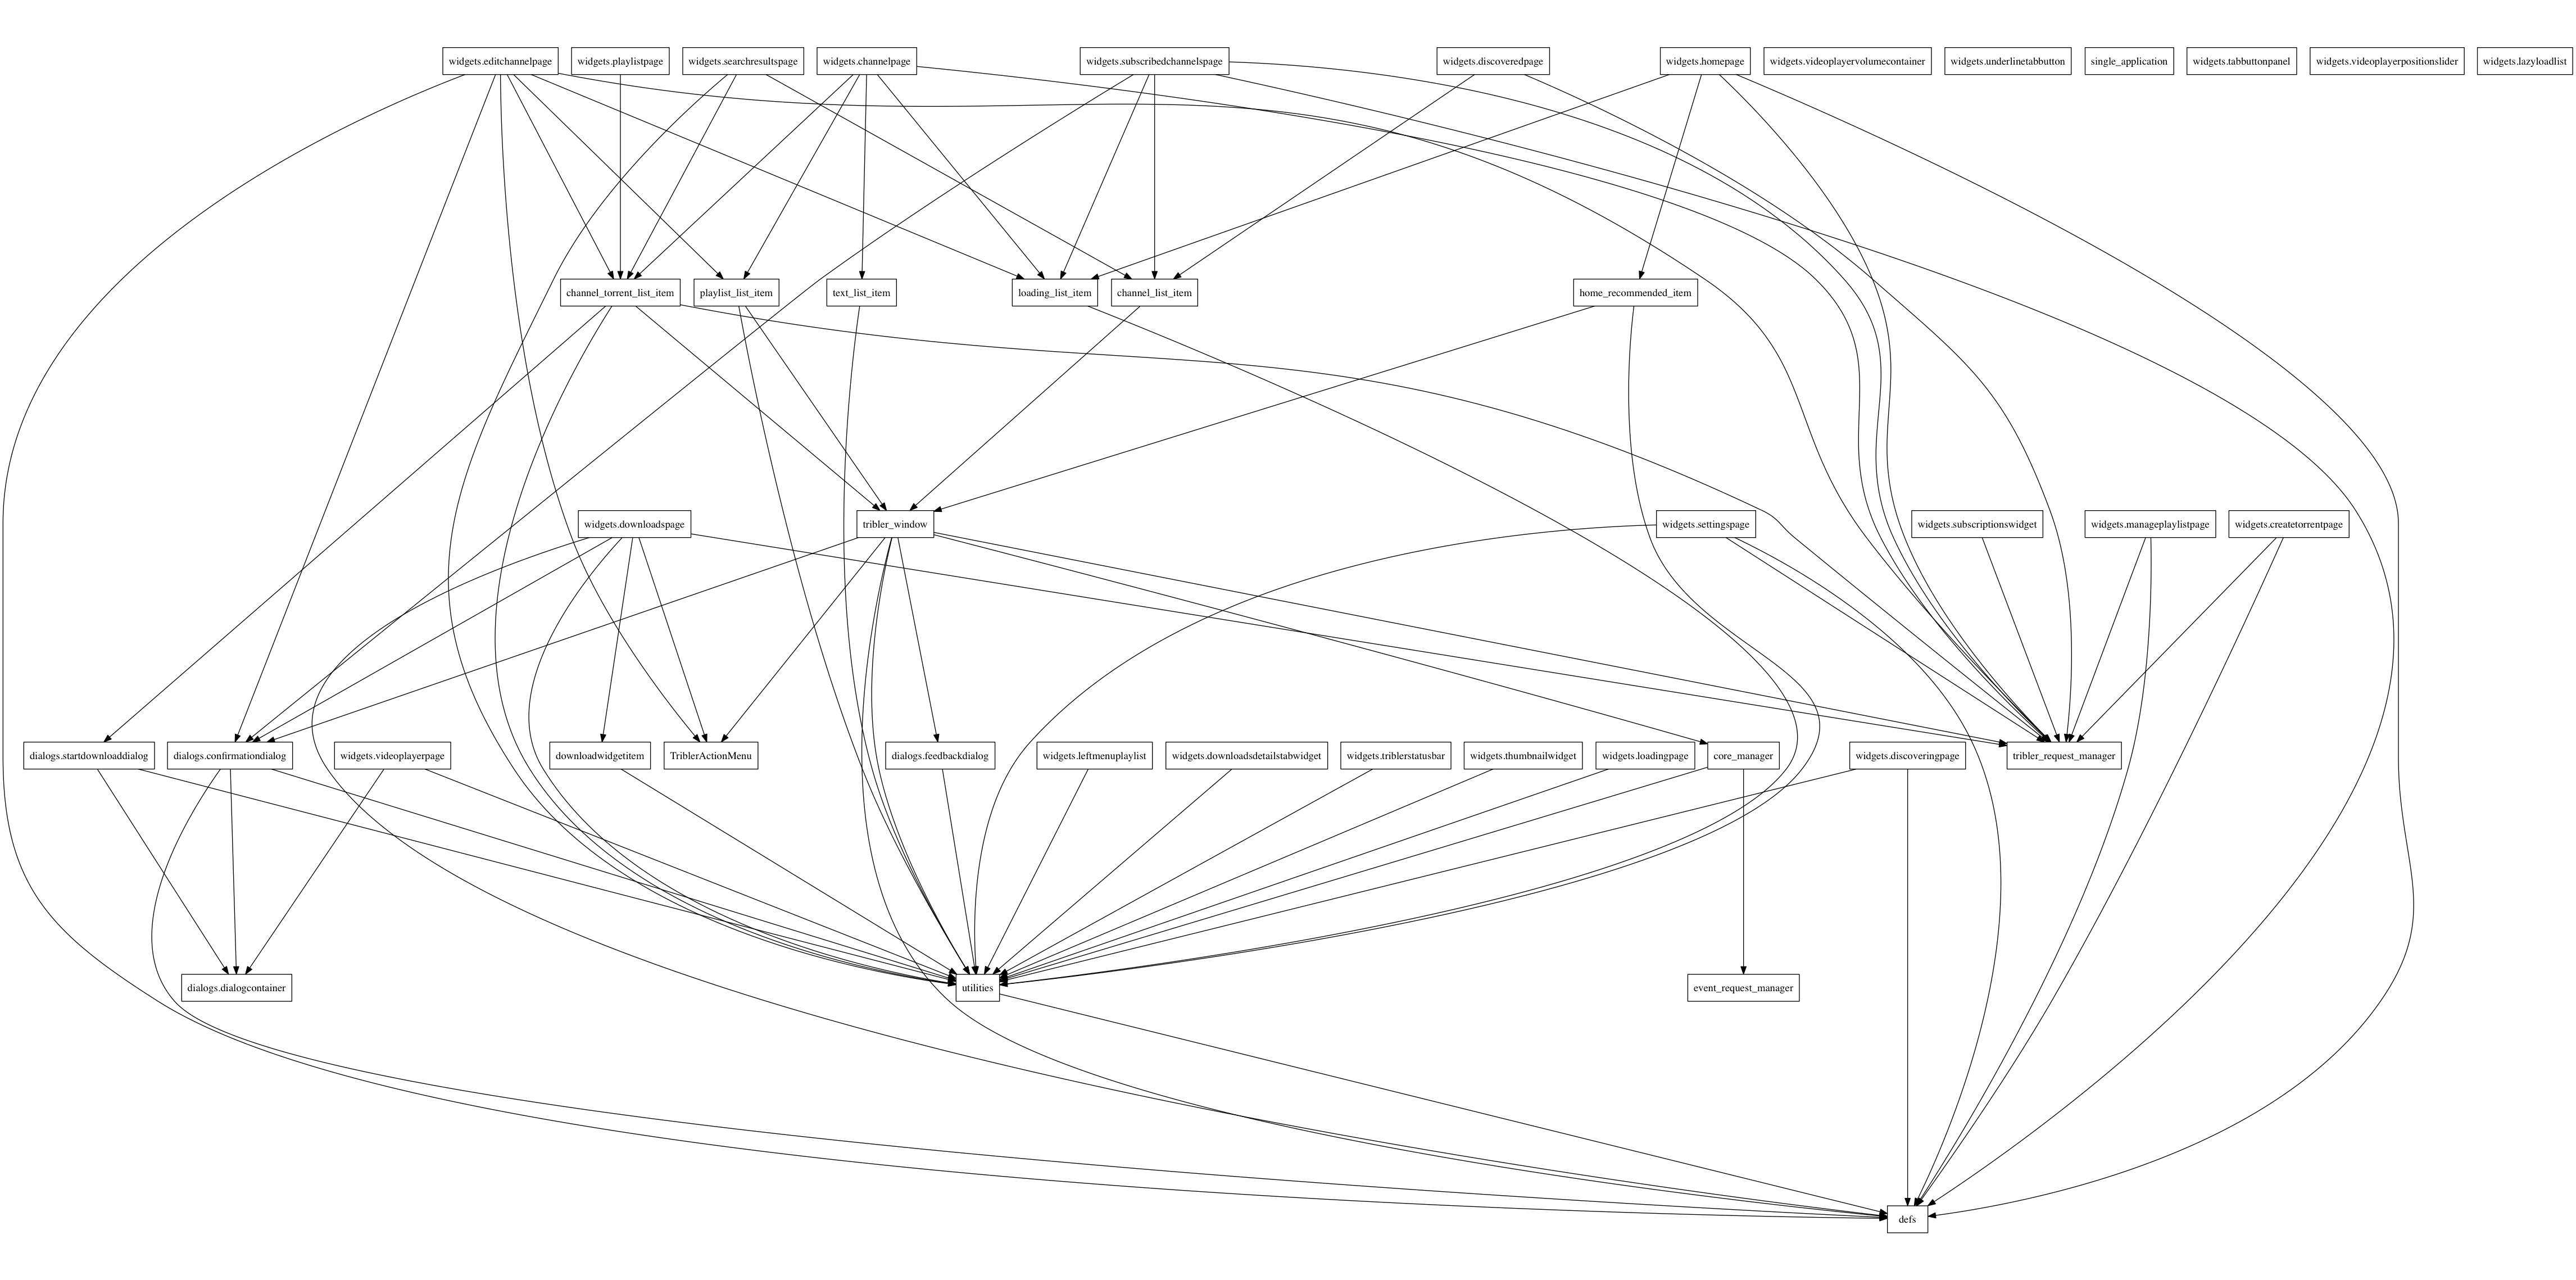
\includegraphics[width=1.0\columnwidth]{images/improving_qa/importgraph_new_gui}
	\caption{The generated import graph of the code base related to the new user interface.}
	\label{fig:importgraph-qt-gui}
\end{figure}

\subsubsection{\textbf{Displaying a huge amount of items}}
\emph{Qt} allows to display possibly many items in a simple list. The performance decreases dramatically if custom widgets are rendered in a list, like we are doing. Loading 1.000 of such list items takes several seconds\todo{verify this}. For each item in the list, the associated user interface file has to be loaded, parsed and rendered, possibly many times per second. Channels hold potentially several thousand of torrents which should be displayed in the user interface.\\\\
This problem has been solved by using two techniques. The first one is lazy loading: by using a lazy-loading approach where more data is loaded when the user has scrolled through the end of the list, we can postpone and possibly avoid loading the whole list at once. This solution has also been implemented in the interface written in \emph{wxPython}. By loading only a subset of the list rows, the user experience can be significantly increased since users don't have to wait until the whole list of items is loaded. The implementation of this lazy-loading solution is reusable and can be found in the \emph{lazyloadlist.py} source file. This however, still resulted in a minor period of waiting when the next set of items is being loaded. It turned out that loading the interface definition file every time is a time-consuming operation. The implemented solution to reduce this processing time is to pre-load the interface definition as soon the user interface starts. This has only a minor effect on the total startup time\todo{hoeveel?}.

\subsubsection{\textbf{A working VLC on multiple platform}}
The old user interface made use of the VLC library for the implementation of the embedded video player. This embedded video player did not function on OS X due to incompatibilities with the wx library used for the implementation of the old interface.

\section{Improvements to the threading model and performance}
The work as described in the last two sections, has led to a better and stable threading model. The complex threading model as used by Tribler 6 is vulnerable for bad code practices, leading to confusion and race conditions. The old threading model is visible in Figure \ref{fig:old-threading-model}. In most Twisted applications, the reactor runs on the main thread of the Python application. In Tribler, the reactor runs on a separate thread since our main thread is occupied by the \emph{wxPython} main loop. User interface-related code such as refresh operations of lists, should always be executed on the Python main thread. Twisted operations however, should be scheduled on the reactor thread. The Twisted threadpool provides some additional threads to dispatch work to and can be used for longer-running operations that should not block the main or reactor thread. Several method decorators have been introduced to make thread switching much easier to implement. These decorators are also visible in Figure \ref{fig:old-threading-model}.\\

\begin{figure}[h!]
	\centering
	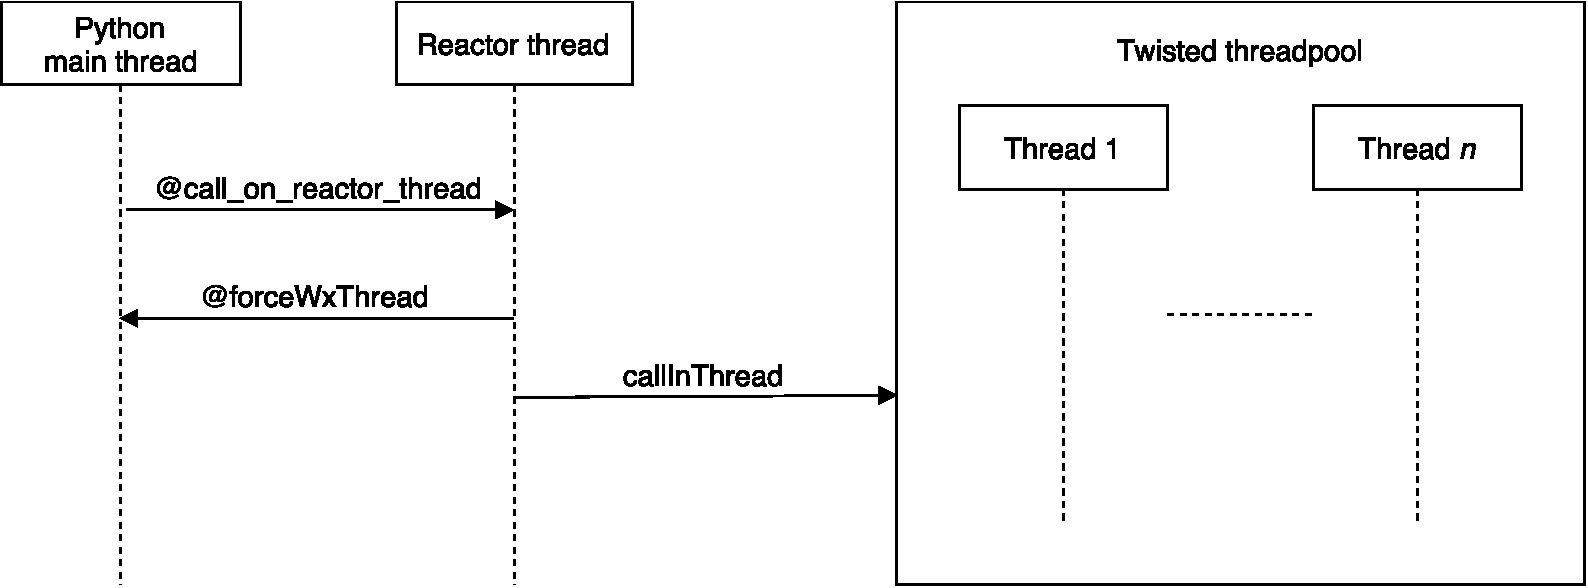
\includegraphics[width=0.9\columnwidth]{images/improving_qa/threading_model_tribler}
	\caption{The threading model in Tribler 6, together with the primitives to schedule operations on different threads.}
	\label{fig:old-threading-model}
\end{figure}

Developers should be aware of the threading context when implementing new features. Long blocking calls on the main thread should be avoided as much as possible since they lead to an unresponsive user interface. Database calls however, should be scheduled on the reactor thread. This threading model leads to much unnecessary confusion and is prone to errors.\\\\
Developing the new user interface came with an additional advantage. Now that the user interface runs in a separate process, we have the opportunity to run the reactor on the main thread. This allows us to get rid of the confusing decorators since we only have one thread (besides the threadpool) to schedule calls on. Getting rid of the abundant thread switching should increase performance since we avoid overhead introduced by the context switch.

\section{Improving Sofware Artifacts}
During the last ten years of development on Tribler, the main focus of the project has been to deliver working code. The project had a severe lack of maintained software artifacts, including documentation, comments and architectural diagrams. Most of the conducted research was documented on the Tribler wiki\footnote{https://www.tribler.org/TitleIndex/}, however, this wiki is very outdated and not maintained anymore. After the migration of the project to GitHub, this platform was favoured over continued usage of the Tribler wiki archive.\\\\
At the moment, there are several distinct locations where we store the few software artifacts we have. Documentation is either stored in the GitHub wiki or in the `docs` directory in the Tribler source code. The ideal situation is to have one single, useful location for all generated documents during the process. Many Python projects are using \emph{readthedocs}, a platform to host documentation for free. The hosted documentation should be located in the Tribler repository, in \emph{reStructuredText} (RST) format. By using the Python module Sphinx, a HTML website can be generated from all the available documentation. Sphinx also provides tool for localization of documentation.

\begin{figure}[h!]
	\centering
	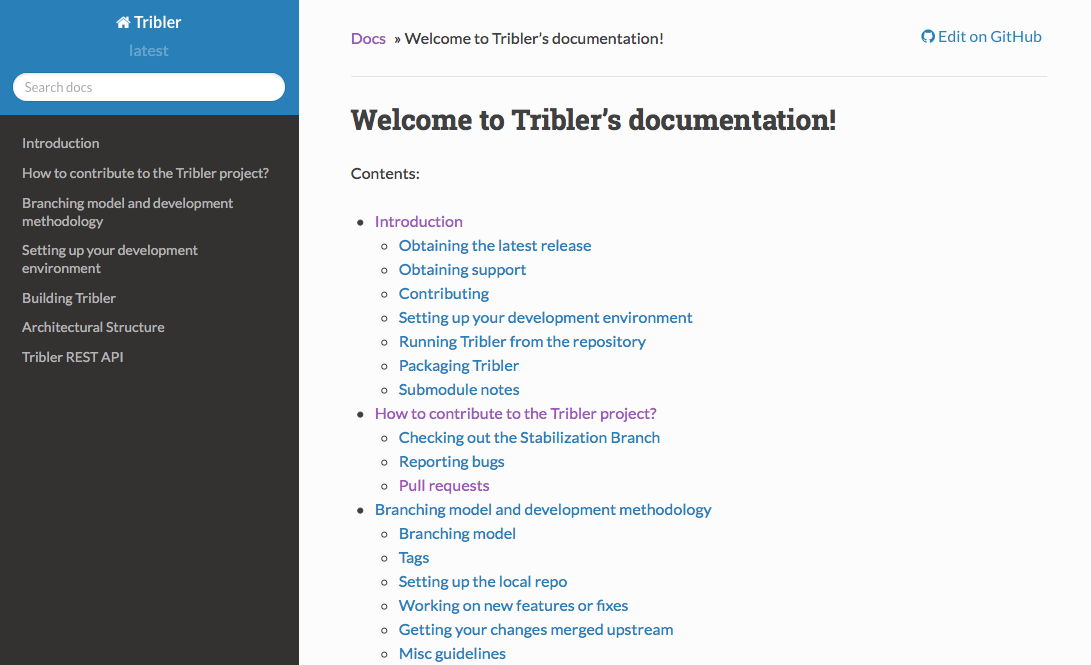
\includegraphics[width=1.0\columnwidth]{images/improving_qa/readthedocs}
	\caption{The documentation of Tribler, as displayed on the \emph{readthedocs} website.}
	\label{fig:old-threading-model}
\end{figure}

During this thesis, all available documentation of Tribler has been rewritten to make use of RST in conjunction with \emph{Sphinx}. Moreover, the available documentation has been improved with several guides, in particular, guides that help users to create a developer environment on their machine. Prior, these guides were not available and development on other platforms than Linux was not supported. By the addition of these guides, new developers can start as soon as possible with development on Tribler.\\\\
The REST API in particular has been very well documented. Since external developers can use the REST API to control Tribler, we wish to provide a clear and comprehensive documentation base for this API. To simplify the process of writing documentation, the documentation can be written as doc strings above each method. The \emph{autosummary} tool that is executed each time the documentation is built, navigates through the API code base, extracts all doc strings and generates page sections for each documented method. The doc string can also be attributed with \emph{RST} syntax. This feature decreases chances that developers accidentally forget to write documentation since the code and documentation is present in the same file instead of being spread across different files.

\begin{figure}[t]
	\centering
	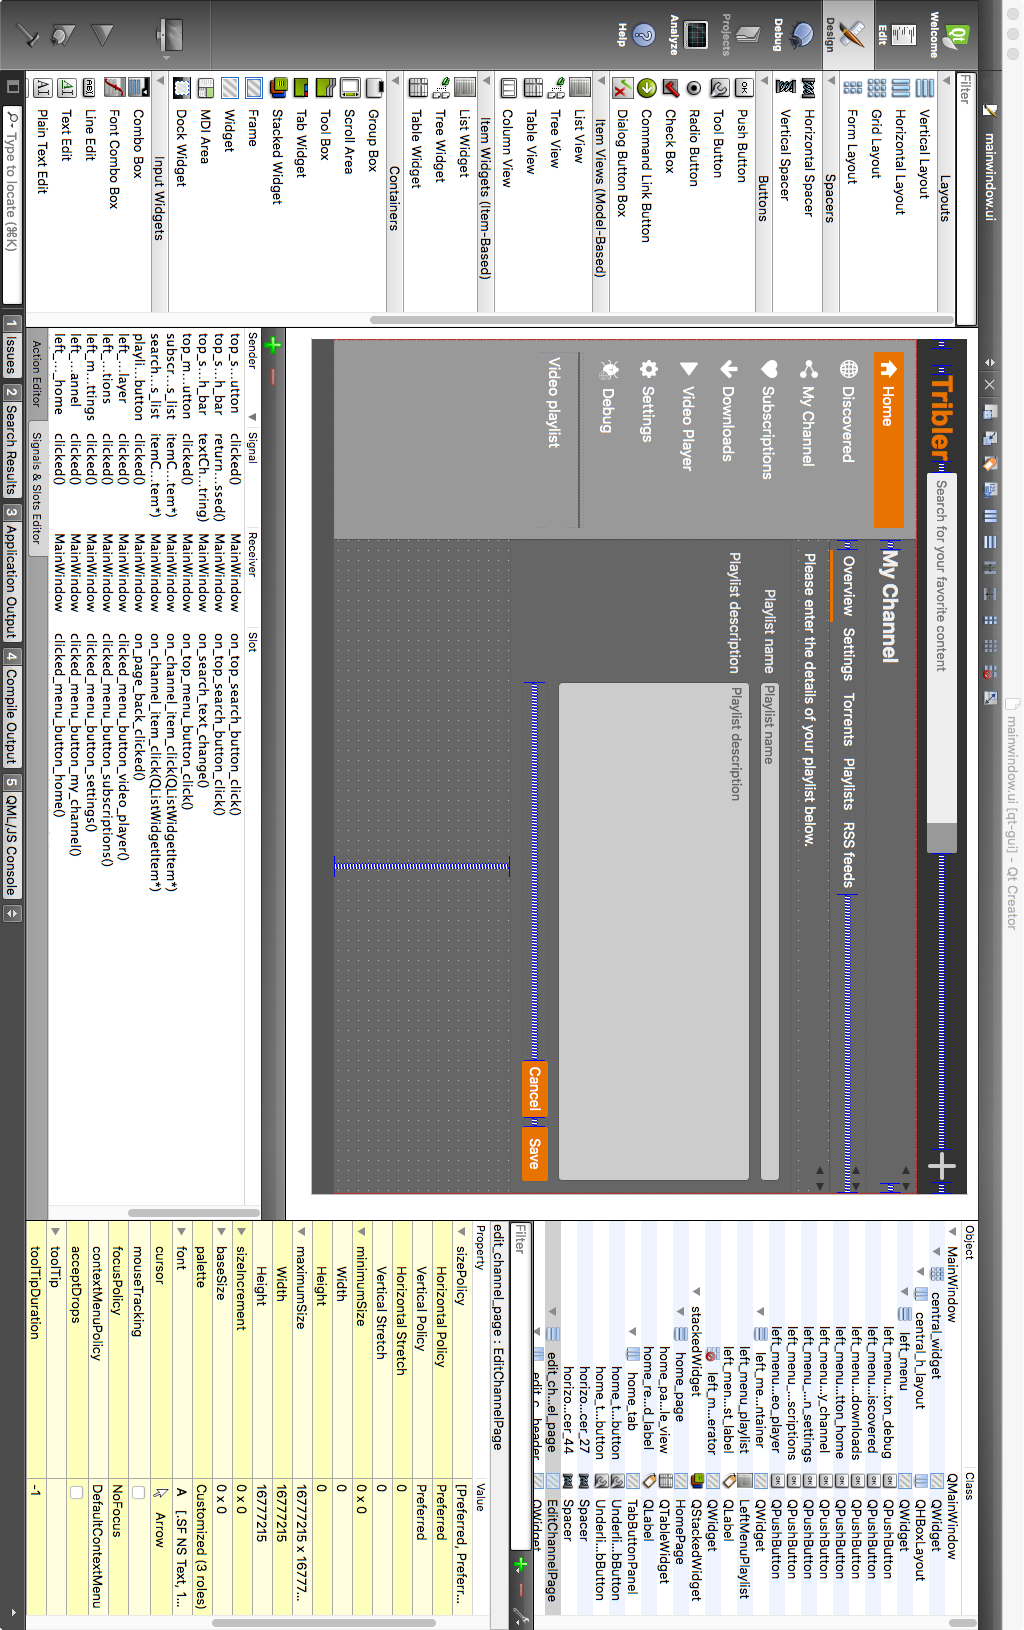
\includegraphics[width=1.0\columnwidth]{images/improving_qa/qt_designer}
	\caption{The Qt visualizer tool used to create the new user interface of Tribler.}
	\label{fig:qt-visualizer}
\end{figure}